\begin{frame}{Robustness Results: GSM8K on different models}

\begin{figure}
\centering
\hspace*{-0.45cm}
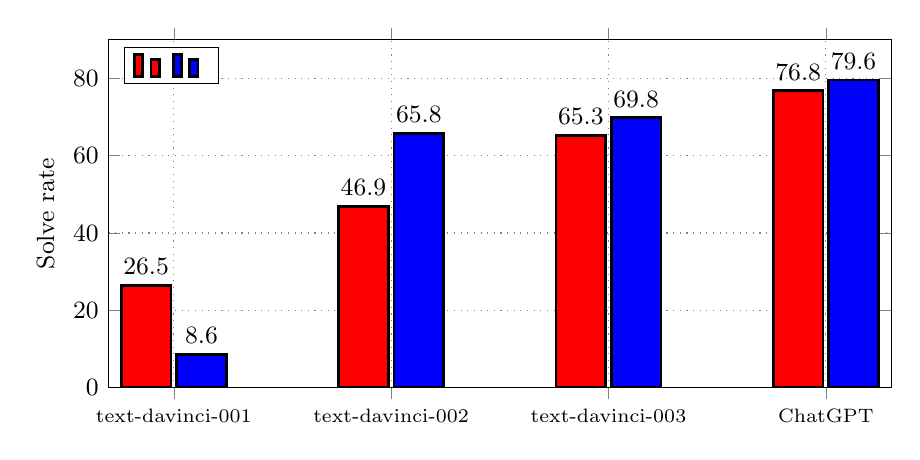
\begin{tikzpicture}
\begin{axis}[
    ybar=2pt,
    bar width=18pt,
    width=0.95\linewidth,
    height=6cm,
    ymin=0,
    ymax=90,
    ytick={0,20,40,60,80},
    ylabel={Solve rate},
    symbolic x coords={
        text-davinci-001,
        text-davinci-002,
        text-davinci-003,
        ChatGPT
    },
    xtick=data,
    xticklabel style={
        font=\scriptsize,
        rotate=0,
        anchor=north
    },
    tick label style={font=\small},
    label style={font=\small},
    legend style={
        at={(0.02,0.98)},
        anchor=north west,
        legend columns=2,
        draw=black,
        fill=white,
        font=\large
    },
    legend cell align={left},
    grid=major,
    major grid style={dotted,gray},
    nodes near coords,
    nodes near coords style={
        font=\small,
        anchor=south
    },
    every axis plot/.append style={
        line width=1pt,
        draw=black
    },
]

\addplot[fill=red] coordinates {
    (text-davinci-001,26.5)
    (text-davinci-002,46.9)
    (text-davinci-003,65.3)
    (ChatGPT,76.8)
};

\addplot[fill=blue] coordinates {
    (text-davinci-001,8.6)
    (text-davinci-002,65.8)
    (text-davinci-003,69.8)
    (ChatGPT,79.6)
};

\legend{\CoT{}, \PAL{}}

\end{axis}
\end{tikzpicture}

\vspace{0.15cm}

\begin{minipage}{0.9\linewidth}
\footnotesize
The GSM8K results show that \PAL{} improves over \CoT{} once the base language model is sufficiently strong. 
For \texttt{text-davinci-001}, \CoT{} performs better, but from \texttt{text-davinci-002} onward, \PAL{} reaches higher solve rates.

\vspace{0.08cm}
{\scriptsize\color{gray}Source: GSM8K benchmark results reported in the PAL paper.}
\end{minipage}

\end{figure}

\end{frame}